%% LyX 2.2.3 created this file.  For more info, see http://www.lyx.org/.
%% Do not edit unless you really know what you are doing.
\documentclass[spanish]{article}
\usepackage[T1]{fontenc}
\usepackage[latin9]{luainputenc}
\usepackage{geometry}
\geometry{verbose,tmargin=2cm,bmargin=2cm,lmargin=2cm,rmargin=2cm,headheight=2cm,headsep=2cm}
\setlength{\parindent}{0bp}
\usepackage{graphicx}

\makeatletter
%%%%%%%%%%%%%%%%%%%%%%%%%%%%%% User specified LaTeX commands.
\usepackage{amsmath}

\makeatother

\usepackage{babel}
\addto\shorthandsspanish{\spanishdeactivate{~<>}}

\begin{document}

\part{Control de tonos y ecualizador de fase}

A lo largo de esta parte, se pondra foco en el circuito mostrado en
la Figura \ref{5_1}, que se trata de un circuito de control de tonos.

\begin{figure}[h]
\begin{centering}
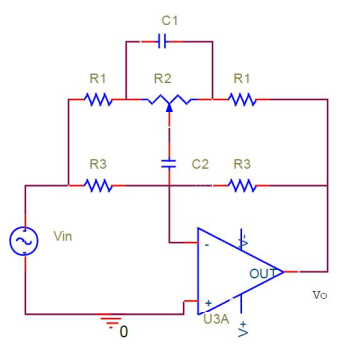
\includegraphics[scale=0.5]{Resources/Circuito}
\par\end{centering}
\caption{Circuito de Control de Tonos}
\label{5_1}

\end{figure}

\section{Transferencia}

Al calcular la transferencia genericamente para cualquier valor de
impedancias, y llamando a $R_{2}=R_{21}+R_{22}$, el calculo de la
transferencia se expresa como la ecuaci�n (\ref{eq:5_1}).

\[
H(s)=-\frac{20C_{2}^{2}K^{2}R_{1}R_{2}^{2}s^{2}-20C_{2}^{2}KR_{1}R_{2}^{2}s^{2}-10C_{2}^{2}R_{1}^{2}R_{2}s^{2}-100C_{2}^{2}R_{1}R_{2}^{2}s^{2}+C_{2}K^{2}R_{2}^{2}s+9C_{2}KR_{2}^{2}s-C_{2}R_{1}^{2}s-31C_{2}R_{1}R_{2}s-10C_{2}R_{2}^{2}s-2R_{1}-R_{2}}{20C_{2}^{2}K^{2}R_{1}R_{2}^{2}s^{2}-20C_{2}^{2}KR_{1}R_{2}^{2}s^{2}-10C_{2}^{2}R_{1}^{2}R_{2}s^{2}-100C_{2}^{2}R_{1}R_{2}^{2}s^{2}+C_{2}K^{2}R_{2}^{2}s-11C_{2}KR_{2}^{2}s-C_{2}R_{1}^{2}s-31C_{2}R_{1}R_{2}s-2R_{1}-R_{2}}
\]

Si reacomodamos de la siguiente manera:

\begin{equation}
H(s)=\frac{As^{2}+Bs+C}{As^{2}+Es+C}\label{eq:5_1}
\end{equation}

\[
A=20C_{2}^{2}K^{2}R_{1}R_{2}^{2}-20C_{2}^{2}KR_{1}R_{2}^{2}-10C_{2}^{2}R_{1}^{2}R_{2}-100C_{2}^{2}R_{1}R_{2}^{2}\approx-100C_{2}^{2}R_{1}R_{2}^{2}
\]

\[
B=C_{2}K^{2}R_{2}^{2}+9C_{2}KR_{2}^{2}-C_{2}R_{1}^{2}-31C_{2}R_{1}R_{2}-10C_{2}R_{2}^{2}
\]

\[
C=-2R_{1}-R_{2}
\]

\[
E=C_{2}K^{2}R_{2}^{2}-11C_{2}KR_{2}^{2}-C_{2}R_{1}^{2}-31C_{2}R_{1}R_{2}
\]

\section{An�lisis de frecuancia central}

Para obtener la frecuencia central, basta con llevar a la ecuaci�n
de transferencia de la siguiente manera

\begin{equation}
H(s)=\frac{\left(\frac{s}{\omega_{0}}\right)^{2}+\frac{s}{Q_{z}\omega_{0}}+1}{\left(\frac{s}{\omega_{0}}\right)^{2}+\frac{s}{Q_{p}\omega_{0}}+1}\label{eq:5_2}
\end{equation}

Por lo tanto;

\[
\frac{1}{\omega_{0}^{2}}=\frac{A}{C}
\]

\[
\Rightarrow\omega_{0}=\frac{\sqrt{2+\frac{R_{2}}{R_{1}}}}{10C_{2}R_{2}}\Longrightarrow f_{0}=\frac{\sqrt{2+\frac{R_{2}}{R_{1}}}}{20\pi C_{2}R_{2}}
\]

\section{An�lisis param�trico}

Si se analiza los factores de calidad correspondientes se obtiene:

\[
Q_{z}=\frac{C}{B\omega_{0}}
\]

\[
Q_{z}=-\frac{10C_{2}\sqrt{R_{1}}R_{2}\sqrt{2R_{1}+R_{2}}}{C_{2}K^{2}R_{2}^{2}+9C_{2}KR_{2}^{2}-C_{2}R_{1}^{2}-31C_{2}R_{1}R_{2}-10C_{2}R_{2}^{2}}
\]

\[
Q_{p}=\frac{C}{E\omega_{0}}
\]

\[
Q_{p}=-\frac{10C_{2}\sqrt{R_{1}}R_{2}\sqrt{2R_{1}+R_{2}}}{-C_{2}K^{2}R_{2}^{2}+11C_{2}KR_{2}^{2}+C_{2}R_{1}^{2}+31C_{2}R_{1}R_{2}}
\]

por lo tanto, la ganancia para la frecuencia central del filtro quedar�
dada por:

\[
A=\frac{R_{1}^{2}+31R_{1}R_{2}+10R_{2}^{2}}{R_{1}\left(R_{1}+31R_{2}\right)}\approx\frac{3R_{1}+R_{2}}{3R_{1}}\,K=0
\]

\[
A=\frac{R_{1}\left(R_{1}+31R_{2}\right)}{R_{1}^{2}+31R_{1}R_{2}+10R_{2}^{2}}\approx\frac{3R_{1}}{R_{2}+3R_{1}}\,K=1
\]

\[
A=\frac{-K^{2}R_{2}^{2}-9KR_{2}^{2}+R_{1}^{2}+31R_{1}R_{2}+10R_{2}^{2}}{-K^{2}R_{2}^{2}+11KR_{2}^{2}+R_{1}^{2}+31R_{1}R_{2}}\,\,\,Expresado\,Parametricamente\,en\,K
\]

\begin{figure}[h]
\begin{centering}
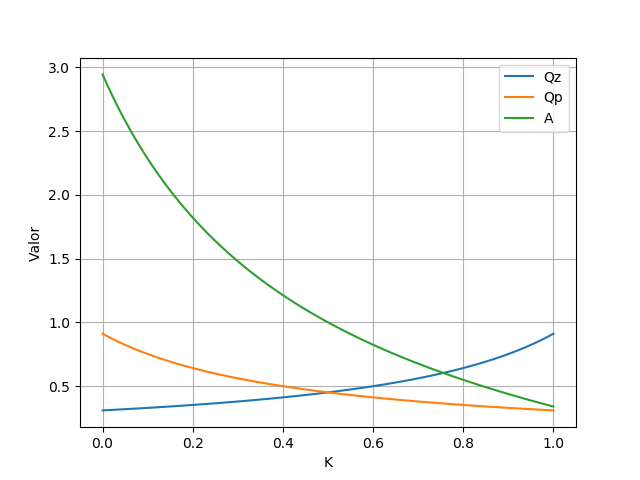
\includegraphics[scale=0.5]{Resources/DiagramaParametrico}
\par\end{centering}
\caption{Diagrama param�trico}

\end{figure}

\begin{figure}[h]
\begin{centering}
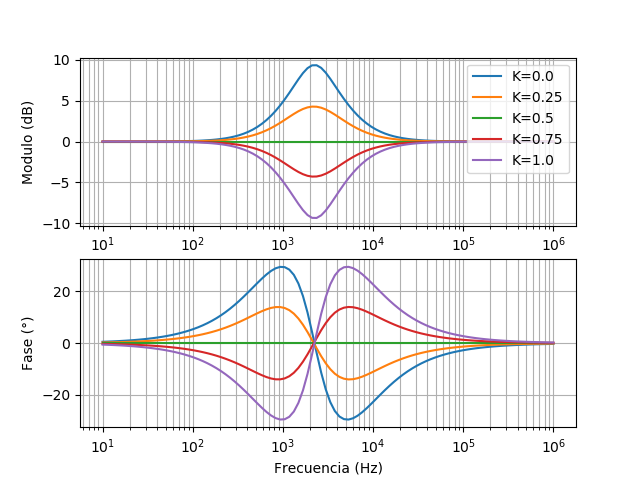
\includegraphics{Resources/RtaEnFrecuanciaParametrica}
\par\end{centering}
\caption{Respuesta en frecuencia param�trica para una frecuencia dada}
\label{5_3}

\end{figure}

\section{An�lisis de singularidades}

\subsection{An�lisis de Ceros\label{subsec:5_4_1}}

Si resolvemos la ecuacion cuadr�tica para el nominador expresado en
la ecuaci�n (\ref{eq:5_2}), obtenemos que la expresi�n para econtrar
los ceros de nuestro circuito, esta dada por:

\[
C_{1,2}=\frac{-\frac{1}{Q_{z}\omega_{0}}\pm\sqrt{\left(\frac{1}{Q_{z}\omega_{0}}\right)^{2}-4\frac{1}{\omega_{0}^{2}}}}{2\frac{1}{\omega_{0}^{2}}}
\]

\[
\Rightarrow C_{1,2}=-\frac{\omega_{0}}{2Q_{z}}\pm\frac{\omega_{0}}{2}\sqrt{\frac{1}{Q_{z}^{2}}-4}
\]

\subsection{An�lisis de polos}

De la misma manera que se procedi� para encontrar los ceros en la
subseccion \ref{subsec:5_4_1}, los polos quedan determinados por:

\[
\Rightarrow P_{1,2}=-\frac{\omega_{0}}{2Q_{P}}\pm\frac{\omega_{0}}{2}\sqrt{\frac{1}{Q_{P}^{2}}-4}
\]

\subsection{An�lisis de singularidades param�tricas}

Si tenemos en cuenta, las expresiones para los pollos y los ceros
obtenidas anteriormente, y una frecuencia central determinada, como
por ejemplo la propuesta en la Figura \ref{5_3}, se podra hacer una
analisis parametrico graficando como var�an los polos y los ceros
en un diagrama Imaginario/Real segun la variaci�n de la resistencia
$R_{2}$.

\begin{figure}[h]
\begin{centering}
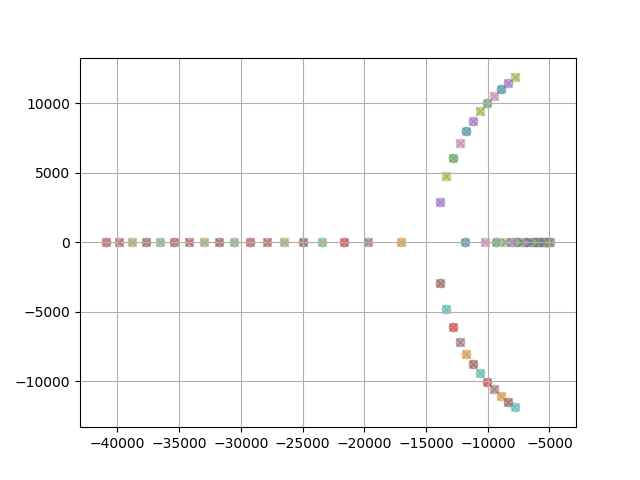
\includegraphics[scale=0.7]{Resources/DiagramaDePolosYCerosCompleto}
\par\end{centering}
\caption{Diagrama param�trico de polos y ceros}
\label{5_4}
\end{figure}

Como se puede observar en la Figura \ref{5_4}, los polos y los ceros
se superponen a partir de cierto valor de K. Graficando los polos
y los ceros con K variando entre $0<K<0.5$ , se obtienen todos los
ceros reales, copmo se puede observar en la Figura \ref{5_5}. Por
otro lado, si se var�a K entre $0.5<K<1$, se puede observar que todos
los polos son reales, como se observa en la Figura \ref{5_6}.

\begin{figure}[h]
\begin{centering}
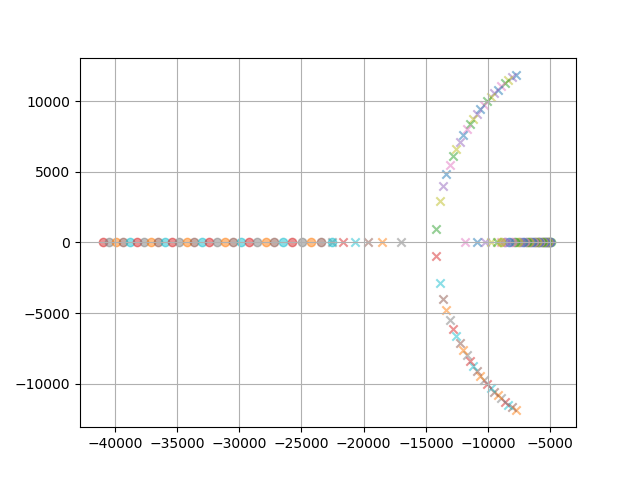
\includegraphics[scale=0.7]{Resources/DiagramaDePolosYCerosHasta05}
\par\end{centering}
\caption{Diagrama param�trico de polos y ceros con K variando de 0 a 0.5}
\label{5_5}

\end{figure}

\begin{figure}[h]
\begin{centering}
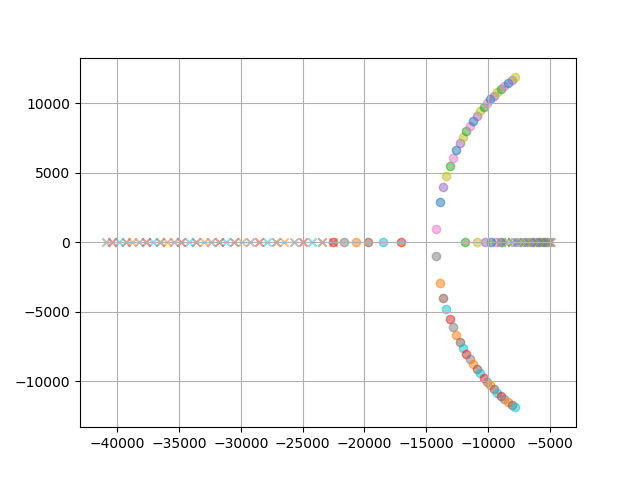
\includegraphics[scale=0.7]{Resources/DiagramaDePolosYCerosDesde05}
\par\end{centering}
\caption{Diagrama param�trico de polos y ceros con K variando de 0.5 a 1}
\label{5_6}
\end{figure}

\end{document}
